% !TEX program  = xelatex

\documentclass{article}
\usepackage{ctex}
\usepackage{xeCJK}
\usepackage[ruled,vlined,linesnumbered]{algorithm2e}
\usepackage{algpseudocode}
\usepackage{amsmath}
\usepackage{amsthm}
\usepackage{graphicx}
\usepackage{subfigure}
\usepackage{float}
\usepackage{amsmath }
\usepackage{amsfonts }
\usepackage{pdfpages}
\usepackage{epsfig}
\usepackage{graphicx}
\usepackage{arydshln}
\usepackage{verbatim}
\usepackage{subfigure}
\usepackage{enumerate}
\usepackage{rotating}
\usepackage{threeparttable}
\usepackage{caption}
\usepackage{tikz}
\usepackage{epsfig}
\usepackage{cite}
\usepackage{geometry}
\usepackage{listings}
\usepackage{xcolor}
\usepackage{fontspec}
\usepackage{booktabs}
\usepackage{adjustbox}
\setCJKmainfont{SourceHanSerifCN-Regular.otf}
\geometry{a4paper, top=2.4cm, bottom=2.4cm, left=3.18cm, right=3.18cm}
\usepackage[colorlinks,linkcolor=red]{hyperref}
\linespread{1.2}

\begin{document}
	\title{AU3601~机器人综合实践~课程报告}
	\author{王凯灵 521030910356}
	\date{2024.4.15}
	\maketitle

	\section{系统框架与说明}
		\subsection{问题重述与基本要求}
			本次课程要求使用卡尔曼滤波器作为机器人定位的算法，定位一个使用力控制的圆柱形移动机器人。在本次实验中，根据前期课程所学知识和提供的代码示例，我们进行如下假设：
			\begin{enumerate}
				\label{ass}
				\item 机器人具有简单的前向运动学关系，总是可以正确的根据力控制信号进行移动。
				\item 机器人的传感器能够且仅能在一定的噪声范围内测量两个绝对方向上和障碍物的距离。
			\end{enumerate}

		\subsection{仿真环境与通信}
		    由于文件上传下载不方便，以及延迟等原因，我使用了本地虚拟机配置环境。我使用了基于Ubuntu18.04的ROS Melodic最新版本。

			我们的示例实现主要涉及三个Python文件，其对应的节点在ROS中的关系如图\ref{fig:rosgraph}所示，其中事实上\texttt{perception.py}中还订阅了\texttt{set\_model\_state}节点，但是其作用是画图，并非出于功能性的订阅。其他未列出节点同理。
			
			\begin{figure}[ht]
				\centering
				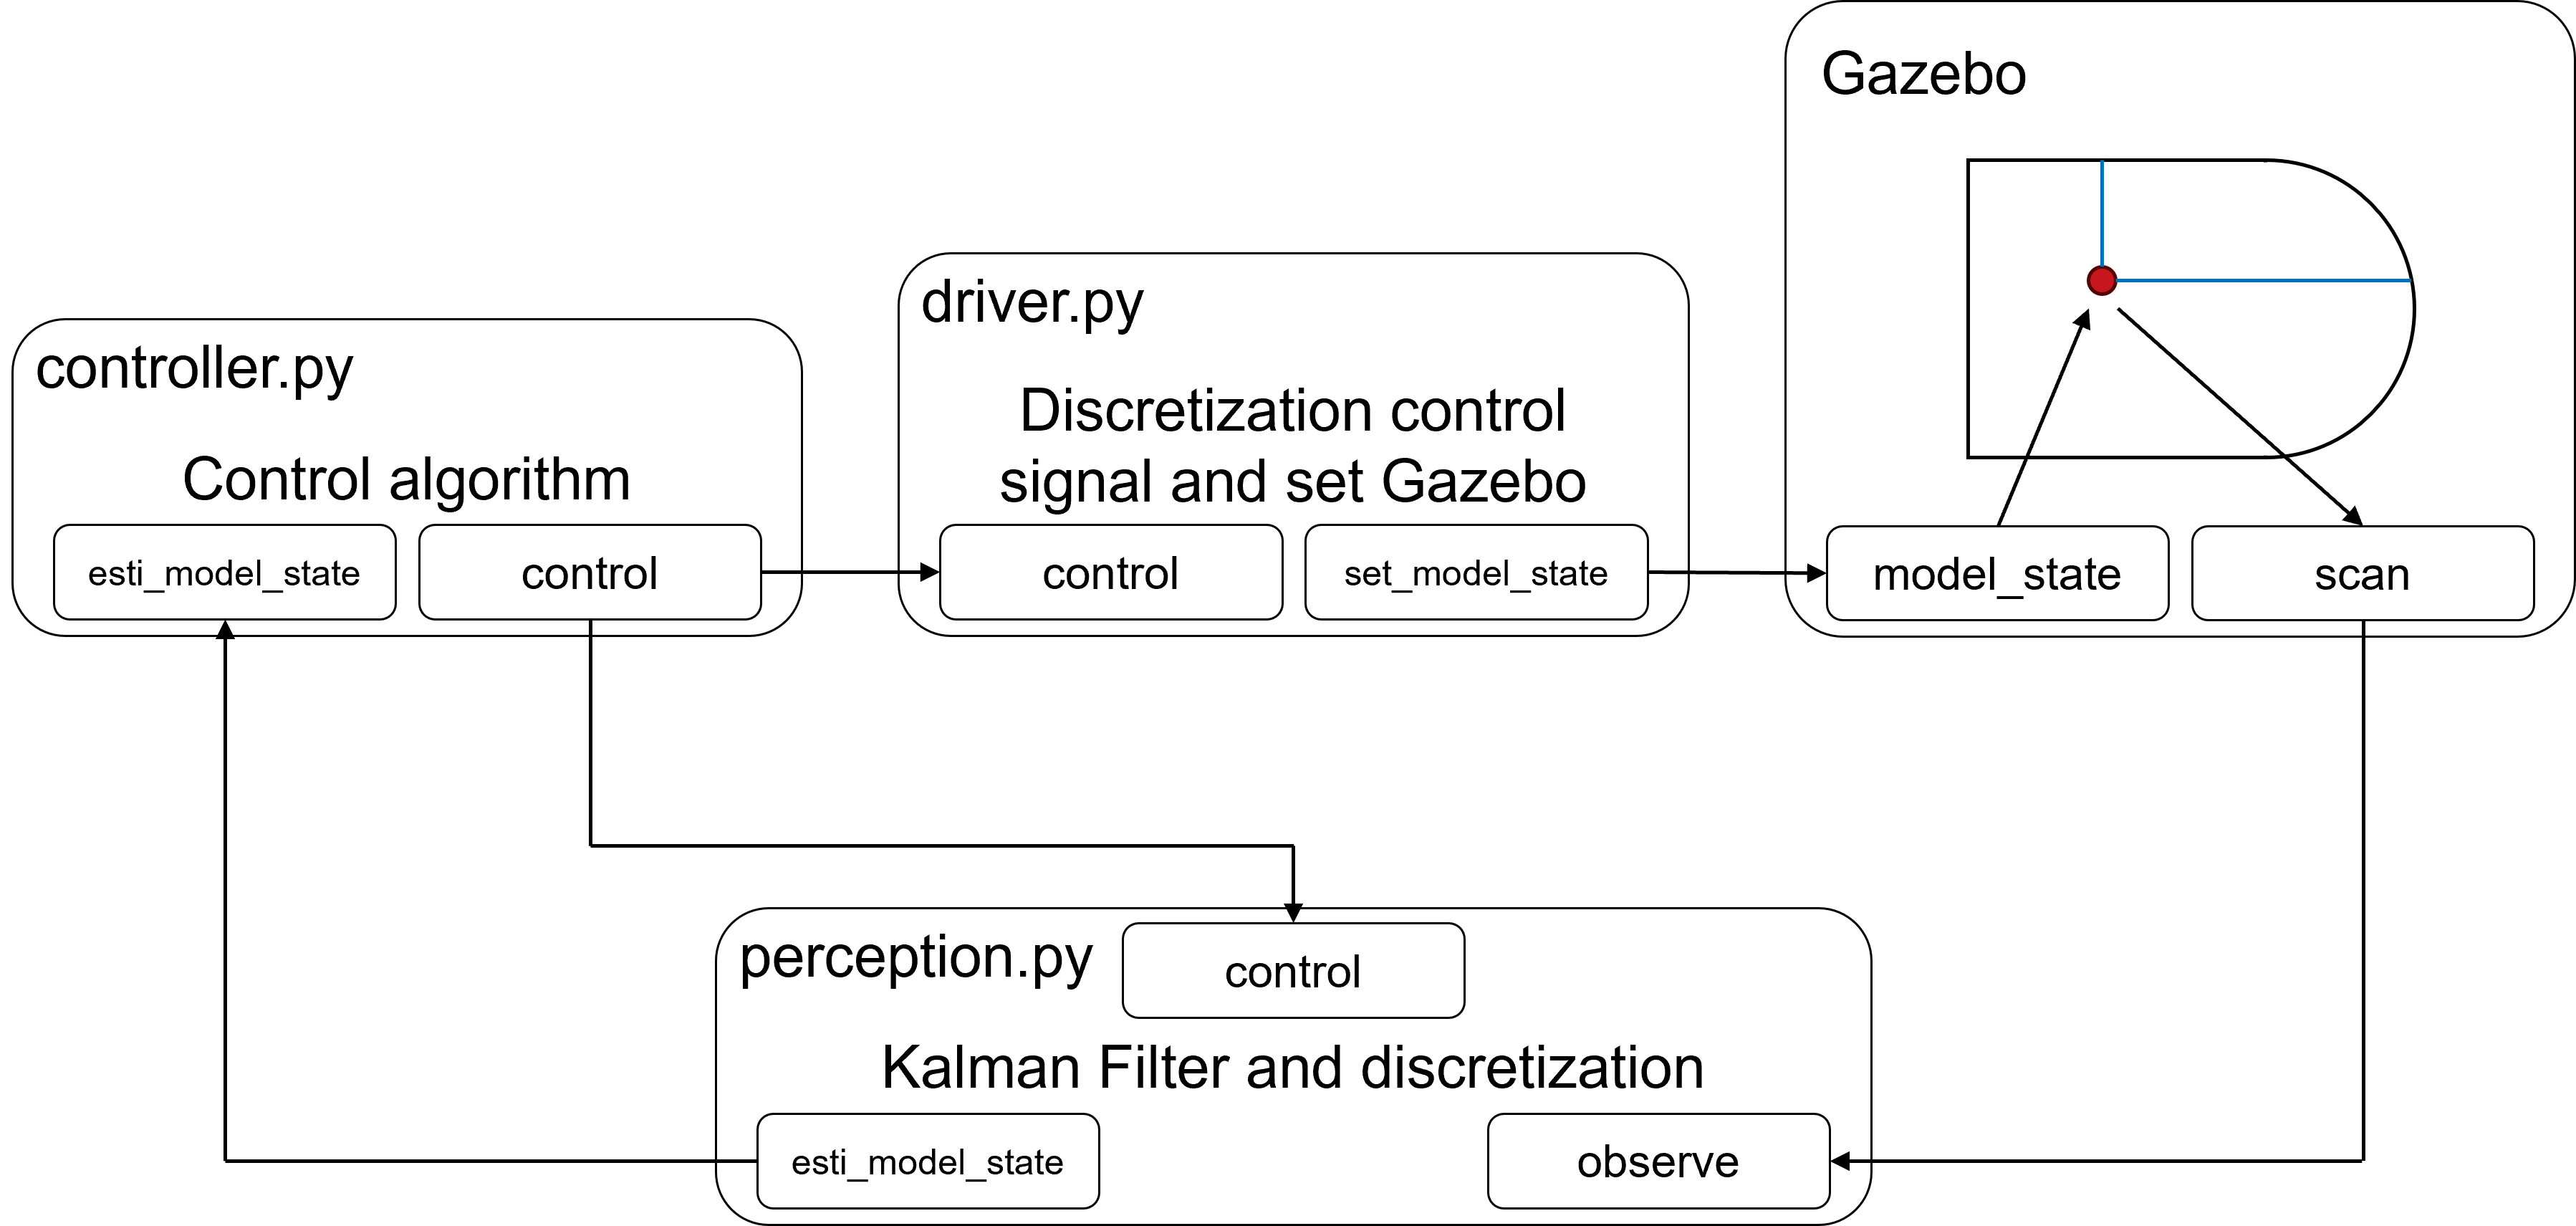
\includegraphics[width=0.9\linewidth]{assets/gazebo_topic}
				\caption{节点关系示意图}
				\label{fig:rosgraph}
			\end{figure}

			所需实现的算法主要在\texttt{controller.py}中，其余部分只需要解决所给模板中的bug或使用前期课程中已完成的实现即可。
		\subsection{物理模型与卡尔曼方程}
			本节将简单重述涉及的物理模型与相应的卡尔曼方程。
			
			基于\ref{ass}中的假设，将机器人看作质点，考虑控制过程中的噪声（对应\texttt{driver.py}），运动学方程为
			
			\[
			\begin{aligned}
				\text{state} : \quad & \mathbf{x} = [v_x, p_x, v_y, p_y]^T \\
				\dot{v}_x &= \frac{F_x}{m} + w_1,~
				\dot{v}_y = \frac{F_y}{m} + w_3\\
				\dot{p}_x &= v_x + w_2,~
				\dot{p}_y = v_y + w_4
			\end{aligned}
			\]
			
			根据课程的推导，经过离散化以后的结果为
			\[
			A = 
			\begin{bmatrix}
				1 & 0 & 0 & 0 \\
				\Delta t & 1 & 0 & 0 \\
				0 & 0 & 1 & 0 \\
				0 & 0 & \Delta t & 1 
			\end{bmatrix},
			\quad
			B = 
			\begin{bmatrix}
				\frac{\Delta t^2}{2m} & 0 \\
				\Delta t & 0 \\
				0 & \frac{\Delta t^2}{2m} \\
				0 & \Delta t
			\end{bmatrix},
			\quad
			\omega_k \sim N(0, \Sigma)
			\]
			
			\[
			\mathbf{x}_{k+1} = A \mathbf{x}_k + B \mathbf{u}_k + \omega_k
			\]
			事实上，从信号的角度来讲，这里的离散化实际上是马尔可夫插值操作，也可以使用窗口多项式拟合，RNN等方法起到类似效果。
			
			卡尔曼方程为
			\[
			\begin{cases}
				\text{状态预测方程：} & \hat{\mathbf{x}}_{k|k-1} = A \hat{\mathbf{x}}_{k-1|k-1} + B \mathbf{u}_{k-1} \\
				\text{预测协方差更新方程：} & P_{k|k-1} = A P_{k-1|k-1} A^T + Q \\
				\text{卡尔曼增益方程：} & K_k = P_{k|k-1} H^T (H P_{k|k-1} H^T + R)^{-1} \\
				\text{状态估计更新方程（测量更新方程）：} & \hat{\mathbf{x}}_{k|k} = \hat{\mathbf{x}}_{k|k-1} + K_k (\mathbf{z}_k - H \hat{\mathbf{x}}_{k|k-1}) \\
				\text{协方差更新方程：} & P_{k|k} = (I - K_k H) P_{k|k-1}
			\end{cases},
			\]
			将上述$A$，$B$带入，所得结果就是所需的质点运动学情景的卡尔曼方程。
		
	\section{实现与说明}
		\subsection{仿真场景的更改}
			场景的可更改部分主要是房间形状，以及障碍物。其中，由于\ref{ass}中已经假设机器人只有两个方向有距离传感器，意味着机器人不能具有实时避障的规划能力，因此也不具有安全的建图方法。而如果地图完全已知，无论如何改变地图形状都没有区别。（注：本课程的同学会在另一课程中被要求实现用于Gazebo中的A*算法，已讨论过该问题）。修改房间以后，只需要修改\texttt{observe}部分的传感器数据到真实坐标的计算即可。墙面非凸或有障碍物的，只需要在传感器跳变点处将坐标转换处理为分段函数即可。
			\begin{figure}[h!]
				\centering
				\begin{minipage}{0.32\textwidth}
					\adjustbox{valign=c}{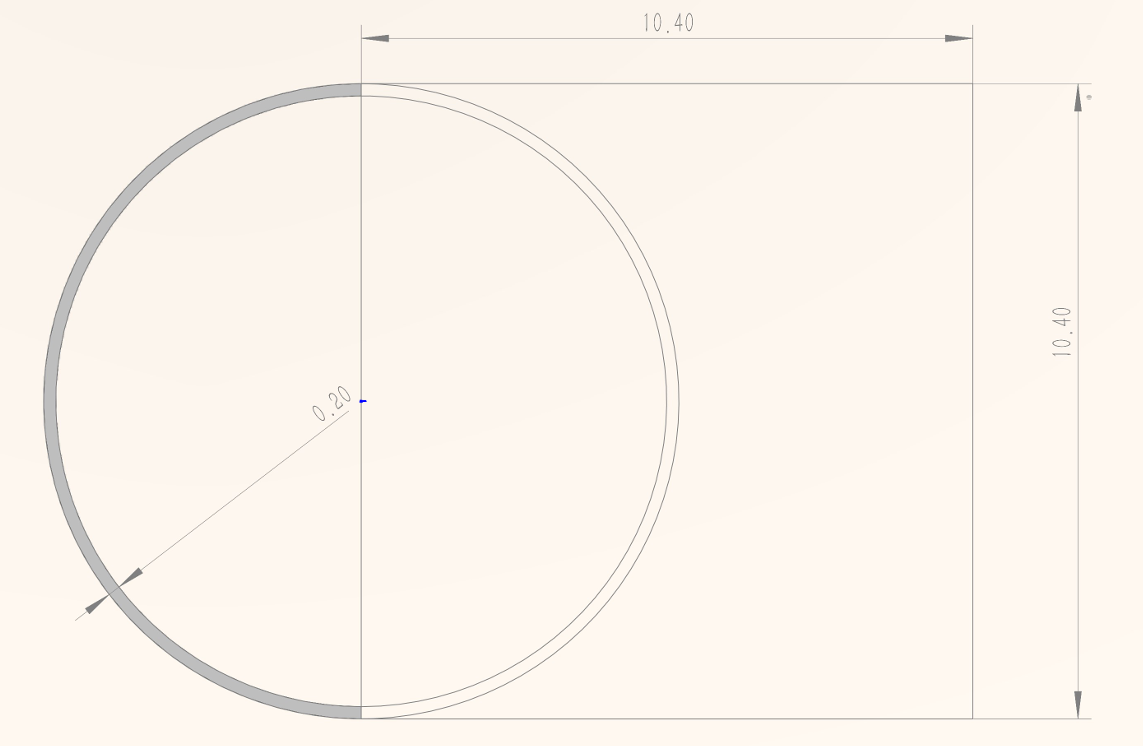
\includegraphics[width=\linewidth]{assets/draft.png}}
				\end{minipage}\hfill
				\begin{minipage}{0.32\textwidth}
					\adjustbox{valign=c}{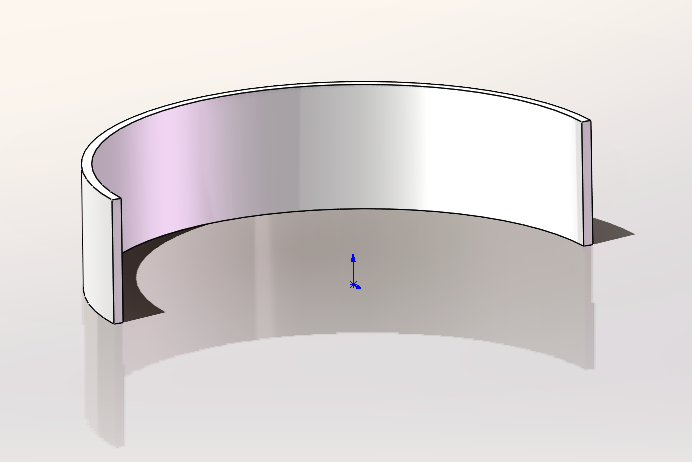
\includegraphics[width=\linewidth]{assets/wall.png}}
				\end{minipage}\hfill
				\begin{minipage}{0.32\textwidth}
					\adjustbox{valign=c}{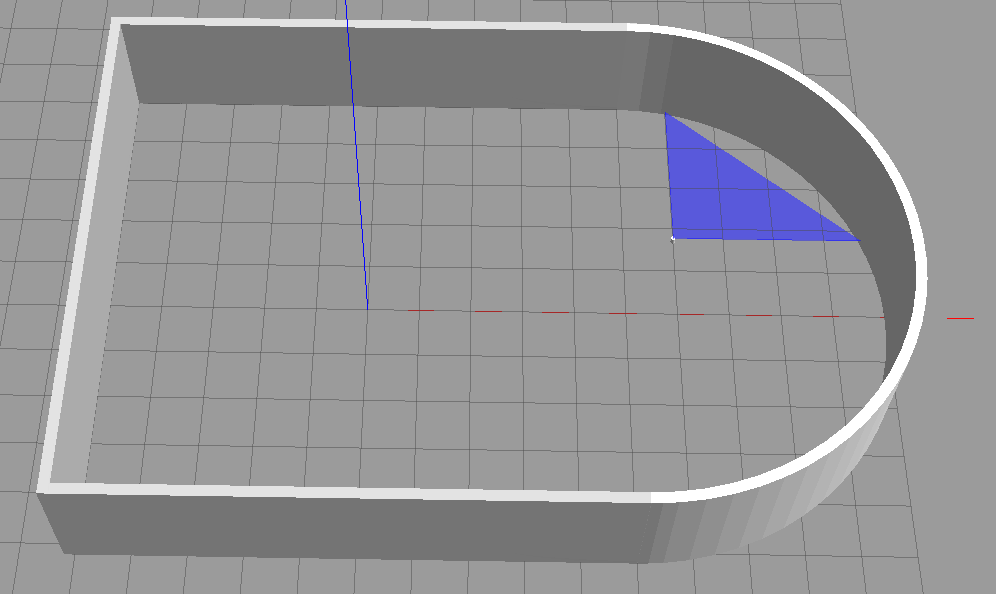
\includegraphics[width=\linewidth]{assets/gazebowall.png}}
				\end{minipage}
				\caption{Gazebo环境模型}
				\label{fig:sw}
			\end{figure}			
			
			Gazebo中只允许使用直线和现有模型进行编辑，所得障碍物只能是直线。为了获得曲线墙面，我在实践过程中速学了简单集合建模，使用SolidWorks进行如图\ref{fig:sw}所示的草图，得到对应墙面。相应的传感器到坐标变换为
			\[
			y = \begin{cases}
				y[0] = 5 - \text{{laserscan.ranges}}[0] + \sqrt{25 - y[1]^2}, \\
				y[1] = 5 - \text{{laserscan.ranges}}[1].
			\end{cases}
			\]
			
		\subsection{实现目的重述}
			在基础要求的基础上，我希望实现一个轨迹跟踪框架。目标轨迹是若干有序点组成的图形轨迹，不一定平滑。轨迹点允许一定范围的误差（0.1单位），机器人只能知道未来的至多2个目标轨迹点，进行实时跟随而不是提前规划。在算法能跟踪轨迹的基础上，我希望实现更优的速度（以跟随用时衡量）、更好的跟随结果（以ATE衡量）。	
		
		\subsection{闭环控制算法}
			本节中将讨论我使用的算法。为了方便比较，我统一使用了三角函数轨迹（公式\ref{sin}）进行可视化。更具体的结果分析将在\ref{results}中具体展开。
			\begin{equation}
				\begin{cases}
					x(t) = \sin(t) \left(4.5 - \frac{t}{10\pi}\right), \\
					y(t) = \cos(t) \left(4.5 - \frac{t}{\pi}\right).
				\end{cases}
				\label{sin}
			\end{equation}
			
			\subsubsection{最简PID控制}
				本场景中，控制变量为机器人的受力，可以视作是加速度控制，而目标是位置或轨迹。离散化的观测变量由卡尔曼滤波提供，包含位置和速度，可以利用速度信号辅助控制。我在早期实现中就PID进行了大量尝试，包括去除I环节，增加微分环节等。 
				
				可用的PID共涉及位置，速度和加速度，控制关系如图\ref{fig:pid}所示。基础的PID只使用位置反馈，其中位置的微分是对速度的约束。所以，完全可以使用速度调节D环节的输出。
				
				图中，速度$v$可以使用速度观测值，将位置微分的目标设为速度观测值，观察上可以在原有PID的基础上减少抖动。这事实上在卡尔曼滤波中引入了负反馈，用估计值约束真实速度，这是本末倒置的行为。如果将图中的$v$定为0，并去掉速度部分的PI环节，这就是所谓的PIDDD形态了。
				
				I环节往往导致超调，在精度要求较高的轨迹跟踪中弊大于利，我在多数尝试中没有使用I环节。
			
				\begin{figure}[ht]
					\centering
					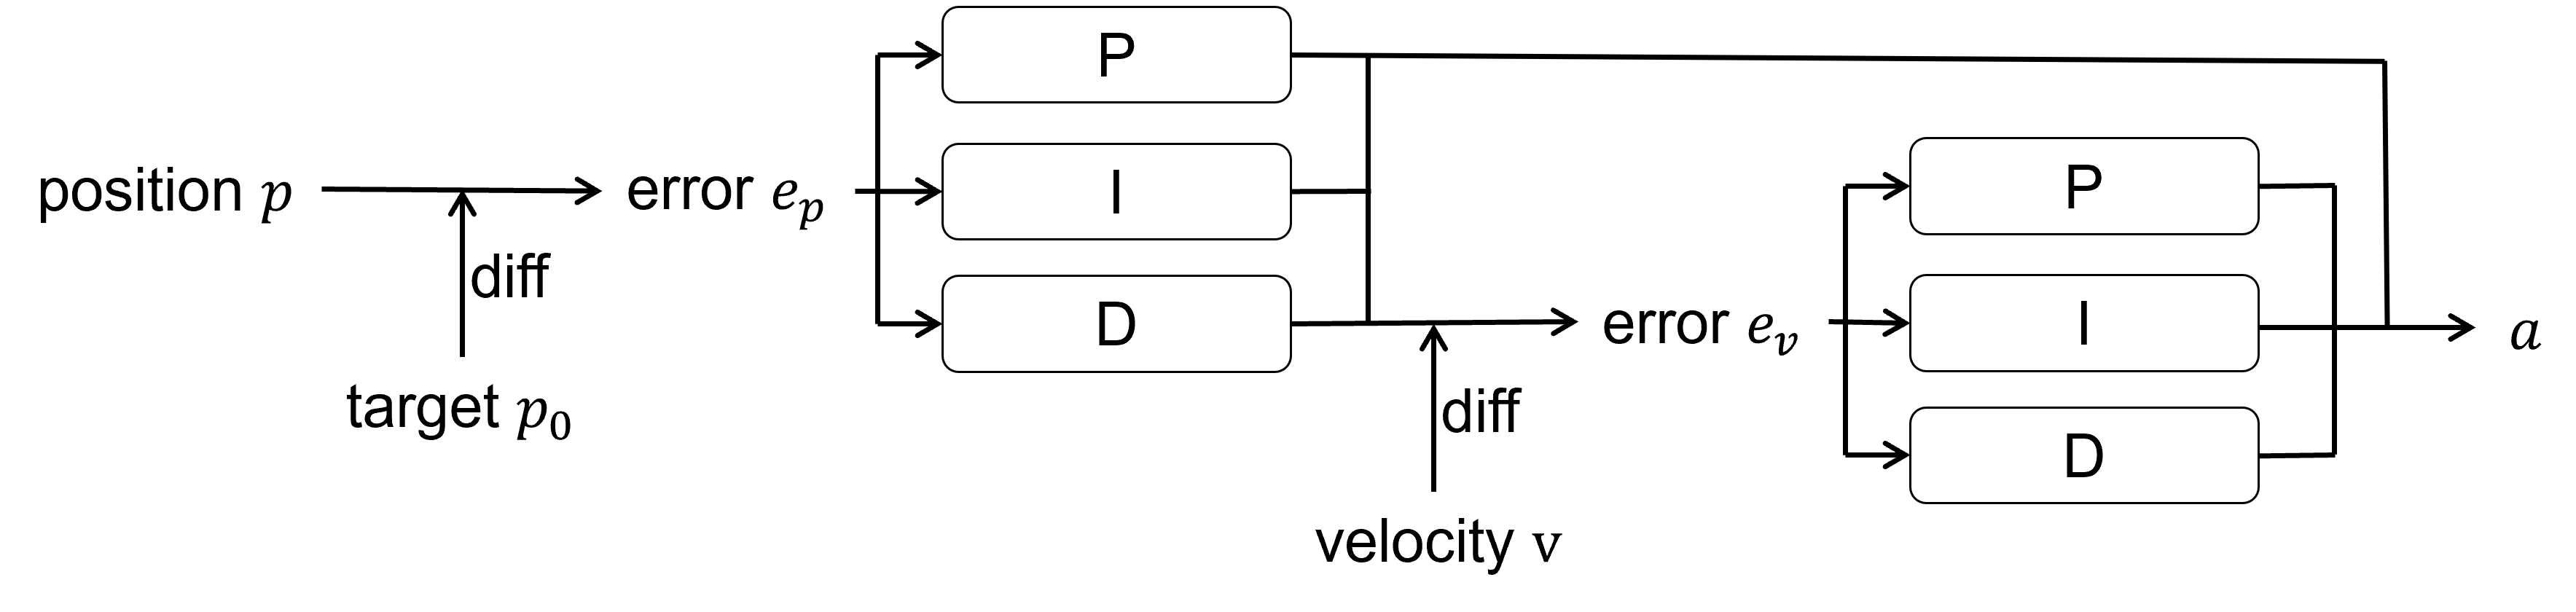
\includegraphics[width=0.9\linewidth]{assets/pidvid}
					\caption{PID变量关系示意图}
					\label{fig:pid}
				\end{figure}
				
				我的PID实现支持了上述框架。在纯PID中，我选择了简单的位置PID和包含0速度的PIDDD控制，效果如图\ref{fig:pidapiddd}所示。初步可见引入DD使得调试难度明显增大，稳定性不如简单的PID。
				
			\begin{figure}[h!]
				\centering
				\begin{minipage}{0.45\textwidth}
					\adjustbox{valign=c}{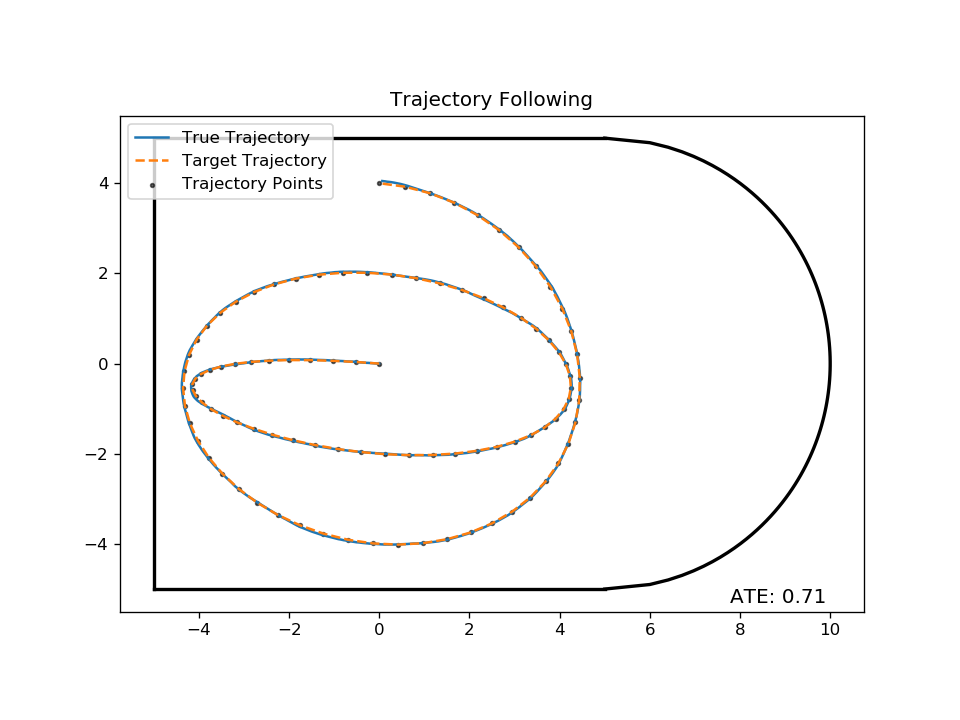
\includegraphics[width=\linewidth]{assets/fig_traj_pid.png}}
				\end{minipage}\hfill
				\begin{minipage}{0.45\textwidth}
					\adjustbox{valign=c}{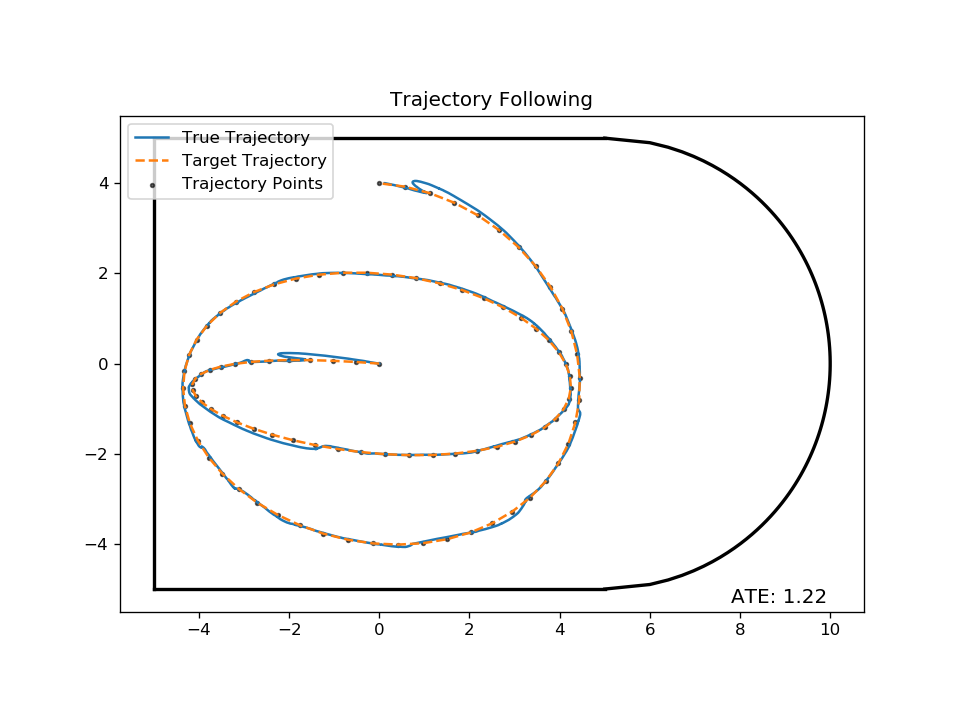
\includegraphics[width=\linewidth]{assets/fig_traj_piddd.png}}
				\end{minipage}
				\caption{PID（左）与PIDDD（右）效果}
				\label{fig:pidapiddd}
			\end{figure}
			
			 \subsection{抛物线控制}
			 	上述的两种PID方法没有对速度的严格约束，速度的不可控会导致轨迹的漂移，容易导致用时和ATE的增加。为了获得更稳定的速度，考虑到基础物理学中，在具有一个加速度的条件下速度不变，最接近的物理模型是平抛运动，考虑使用平抛运动的物理关系作为目标进行控制。
			 	
			 	\begin{figure}[ht]
			 		\centering
			 		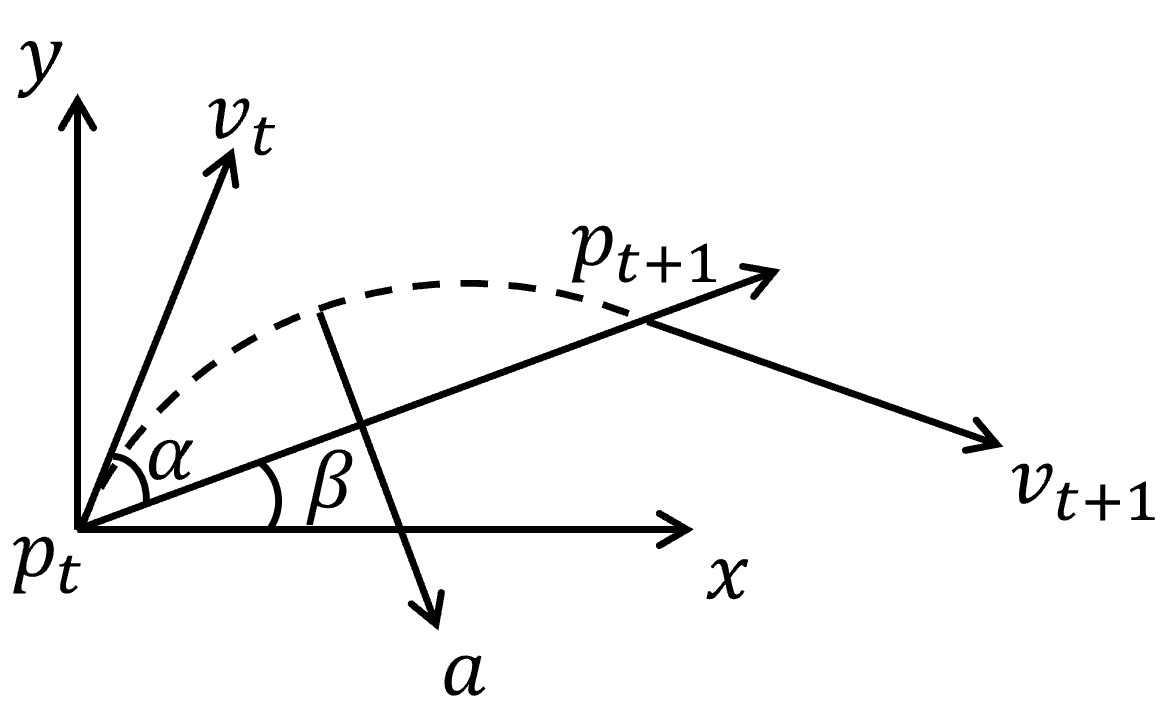
\includegraphics[width=0.5\linewidth]{assets/poly}
			 		\caption{抛物线模型}
			 		\label{fig:poly}
			 	\end{figure}
			 	 
			 	如图\ref{fig:poly}所示，我们希望在经过下一个轨迹点$p_{t+1}$时，速度不变，即$v_t = v_{t+1}$。根据物理学关系，
			 	\begin{align}
			 		\text{令}p_t &= (d_x, d_y), v_t = v_{t+1}=v \text{沿}p_{t+1}-p_t\text{方向分解：}\\
			 		v_\tau &= \frac{v_x d_x + v_y d_y}{\sqrt{d_x^2+d_y^2}}, v_\perp = \frac{v_x d_y + v_y d_x}{\sqrt{d_x^2+d_y^2}}\\
			 		\text{抛物用时}t &= \frac{d_x^2 + d_y^2}{v_x d_y+v_y d_x}\\
			 		\text{计算可得}a &= \frac{v_\perp}{t}\text{,再分解到坐标系即可。}
			 	\end{align}
			 	
			 	使用该项控制加速度，同时使用PID控制速度以免出现累计速度偏移。该方法结果如图\ref{fig:polyacv} 。
			 	
				\begin{figure}[h!]
					\centering
					\begin{minipage}{0.45\textwidth}
						\adjustbox{valign=c}{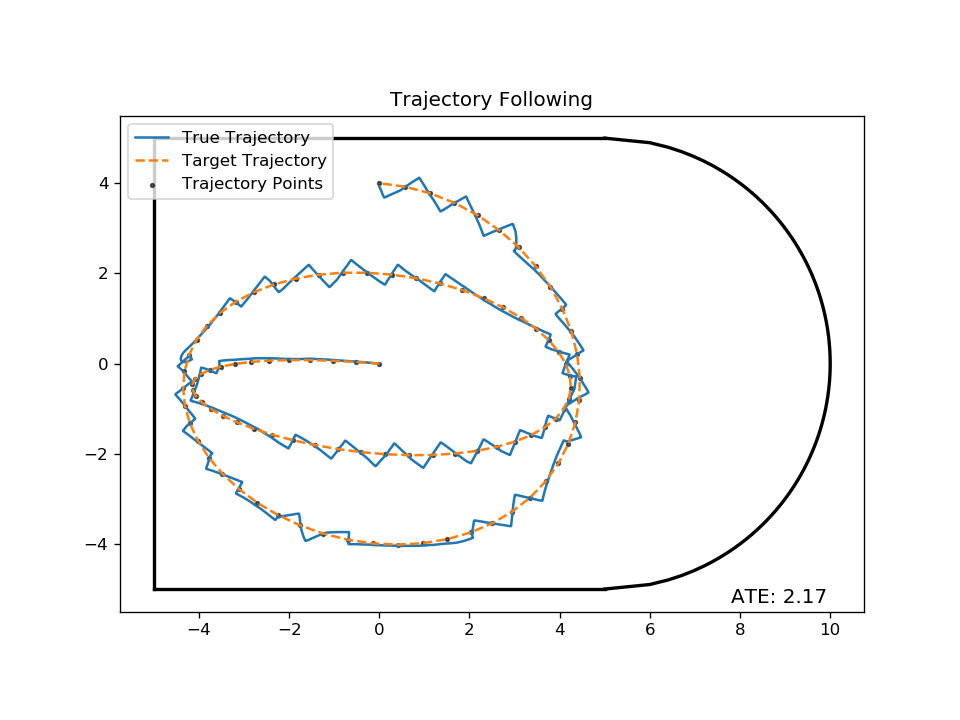
\includegraphics[width=\linewidth]{assets/fig_traj_poly.png}}
					\end{minipage}\hfill
					\begin{minipage}{0.45\textwidth}
						\adjustbox{valign=c}{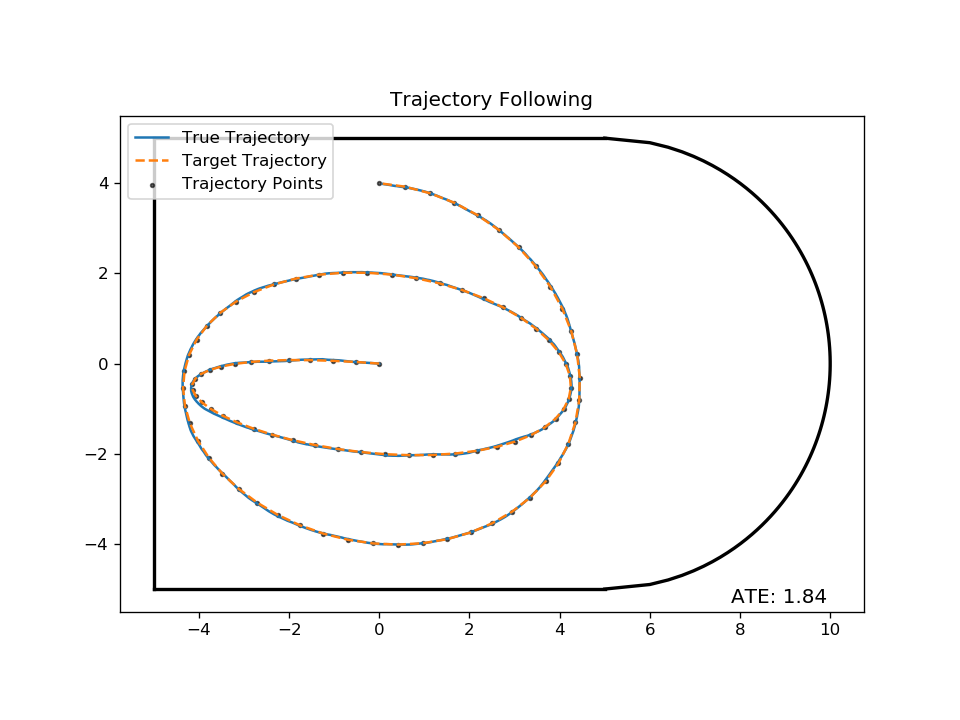
\includegraphics[width=\linewidth]{assets/fig_traj_adv.png}}
					\end{minipage}
					\caption{抛物线（左）与匀速控制（右）效果}
					\label{fig:polyacv}
				\end{figure}
			
			 \subsection{均匀速度控制}
			 	由于常见轨迹的局部大多可以直接使用二阶多项式良好拟合，抛物线方法具有很好的曲线适应性，但再在直线部分和折角部分不能很好跟随，反而会由于抛物线拟合出现期望以外的抖动。
			
				与抛物线不同，匀速控制将速度更改为沿目标点连线方向，即不使用二阶拟合，总是认为未来目标轨迹是直线。该方法示意图为\ref{fig:cv}。然而，该方法没有解决直角转弯问题。进一步引入下一个观测点，将速度方向指向未来的第二个点$p_{t+2}$。如果中间点$p_{t+1}$是折角，则机器人路径将平滑且对称地通过折角。
				\begin{figure}[ht]
					\centering
					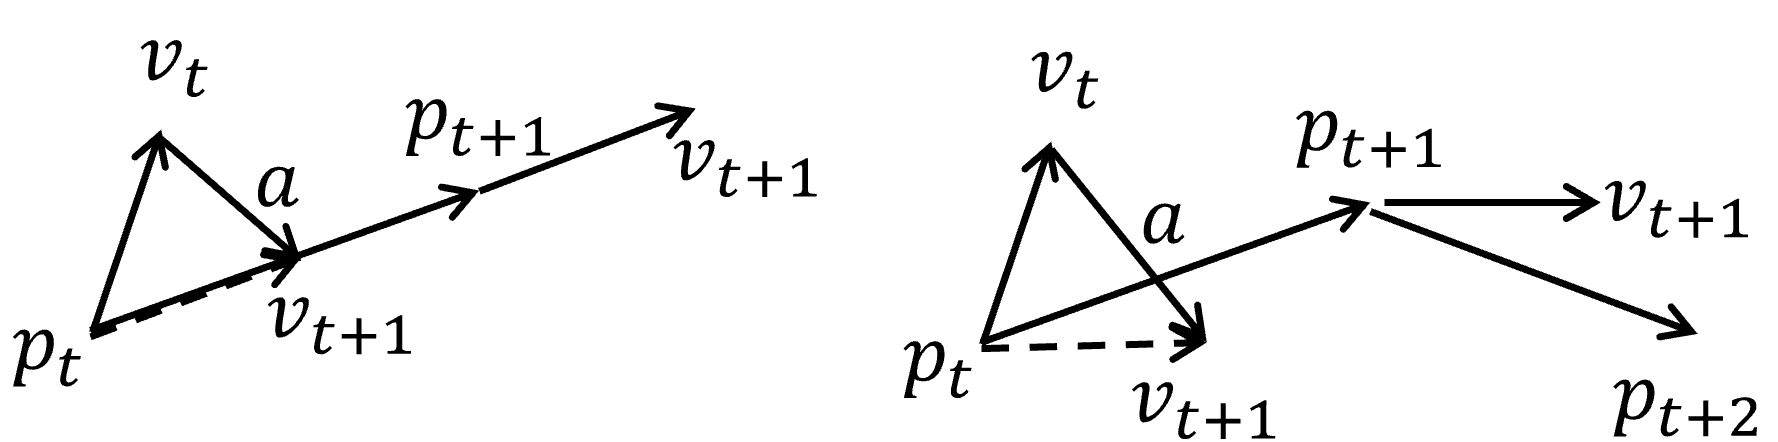
\includegraphics[width=0.7\linewidth]{assets/cv}
					\caption{两点匀速控制（左）和三点匀速控制（右）示意图}
					\label{fig:cv}
				\end{figure}
				
			\subsection{其他问题与解决}
				\begin{itemize}
					\item 实现细节：考虑到机器人需要起步加速等，实现中对速度做了分段处理，分为加速阶段，匀速阶段。其中匀速阶段会使用PID辅助控制，并在误差足够大时直接使用油门刹车（延速度方向的加速度常量）调节速度。实现中包含debug模式，部分信息输出和绘图需要开启debug模式才可见。
					\item 写在最后：可能由于一些适配问题，我使用完全相同的配置，在12代Intel处理器上遇到了极其严重的性能问题。我通过指令单次启动仿真环境需要约20分钟，且可能在中途通信报错退出。我运行的仿真速率大约为2fps，仿真全过程另需约10分钟，即使记录仿真时间也不能保证稳定，导致记录的大量实验时间具有显著随机误差，甚至还因此导致了严重的超调。我直到完成了所有内容才尝试更换机器，发现环境在古老的机器上可以流畅运行。我仅将涉及时间的实验结果进行更新。
				\end{itemize}
			
				
	\section{实验结果}
		\label{results}
		\subsection{基础的卡尔曼滤波结果}
		实现了卡尔曼滤波器的基础版本如图\ref{fig:x}所示。该运动是一个沿着x负方向的先匀加速后匀减速运动。结果显示跟随效果稳定，观测误差在设置值0.02范围内波动，在预期范围内。本实践并未对卡尔曼滤波器本身进行改动。
			\begin{figure}[ht]
				\centering
				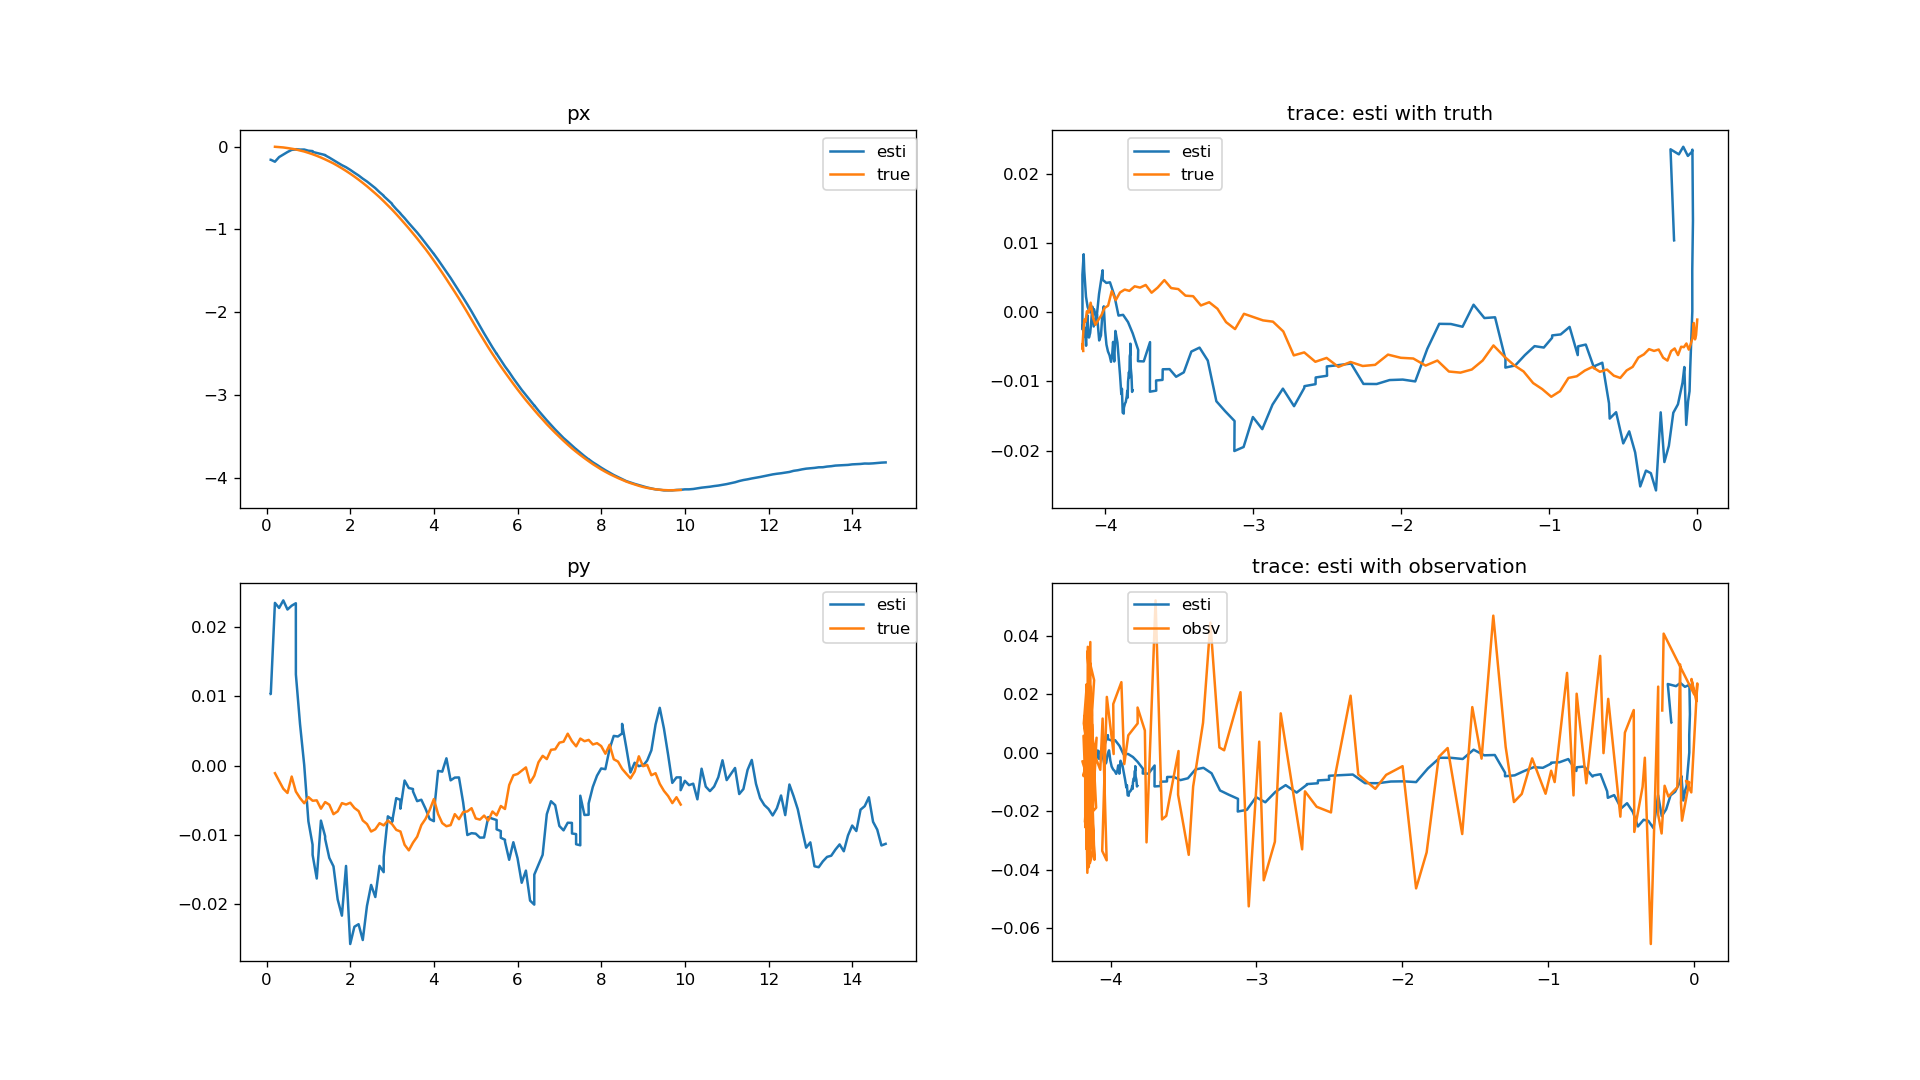
\includegraphics[width=0.9\linewidth]{assets/fig_x}
				\caption{基本运动结果}
				\label{fig:x}
			\end{figure}
			
		\subsection{轨迹跟随结果}
			\subsubsection{及时减速}
				PID类方法和抛物线没有良好的减速机制，所以均在长距离移动时发生了图\ref{fig:wall}（左）的撞墙。匀速控制的假设可以避免这一问题，因为有明确的速度目标。效果如图\ref{fig:wall}（右）。
			
				\begin{figure}[ht]
					\centering
					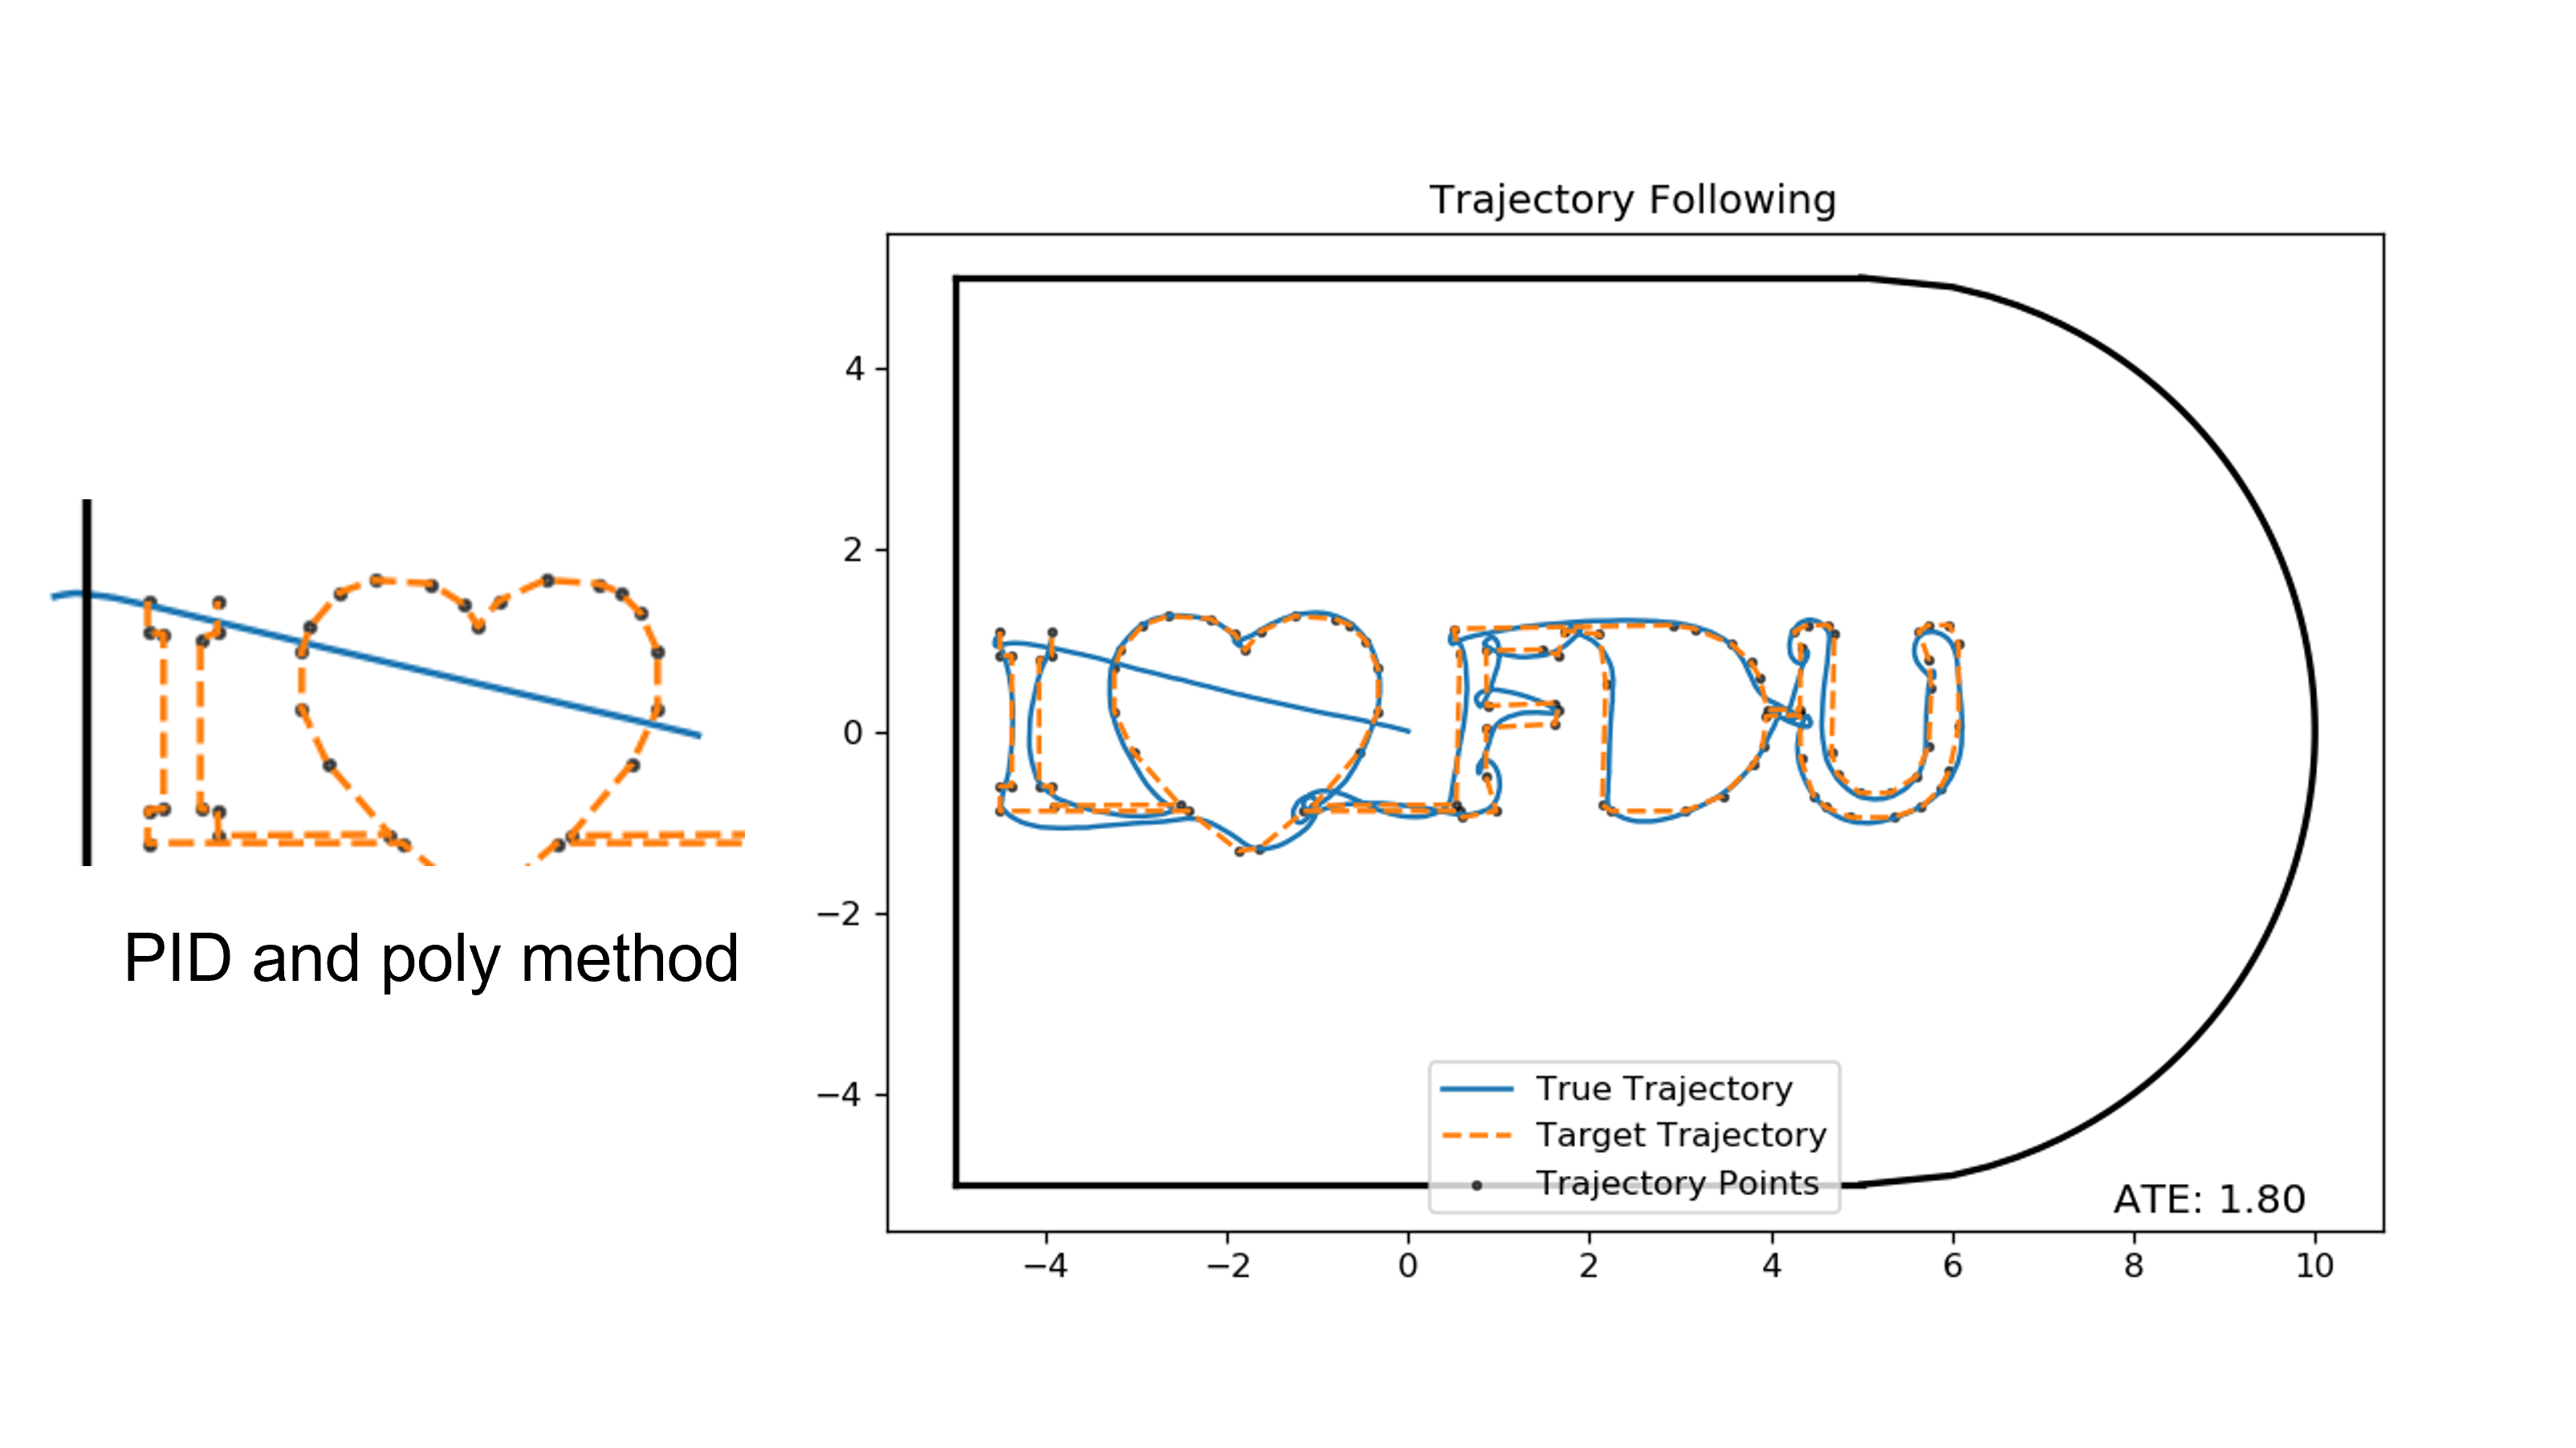
\includegraphics[width=0.65\linewidth]{assets/wallhit}
					\caption{及时减速比较}
					\label{fig:wall}
				\end{figure}
				
			\subsubsection{快速过弯}
				三点匀速控制是为了过弯而设计的。图\ref{fig:corner}展示了相比于PIDDD，三点匀速过急弯的结果。
			
				\begin{figure}[ht]
					\centering
					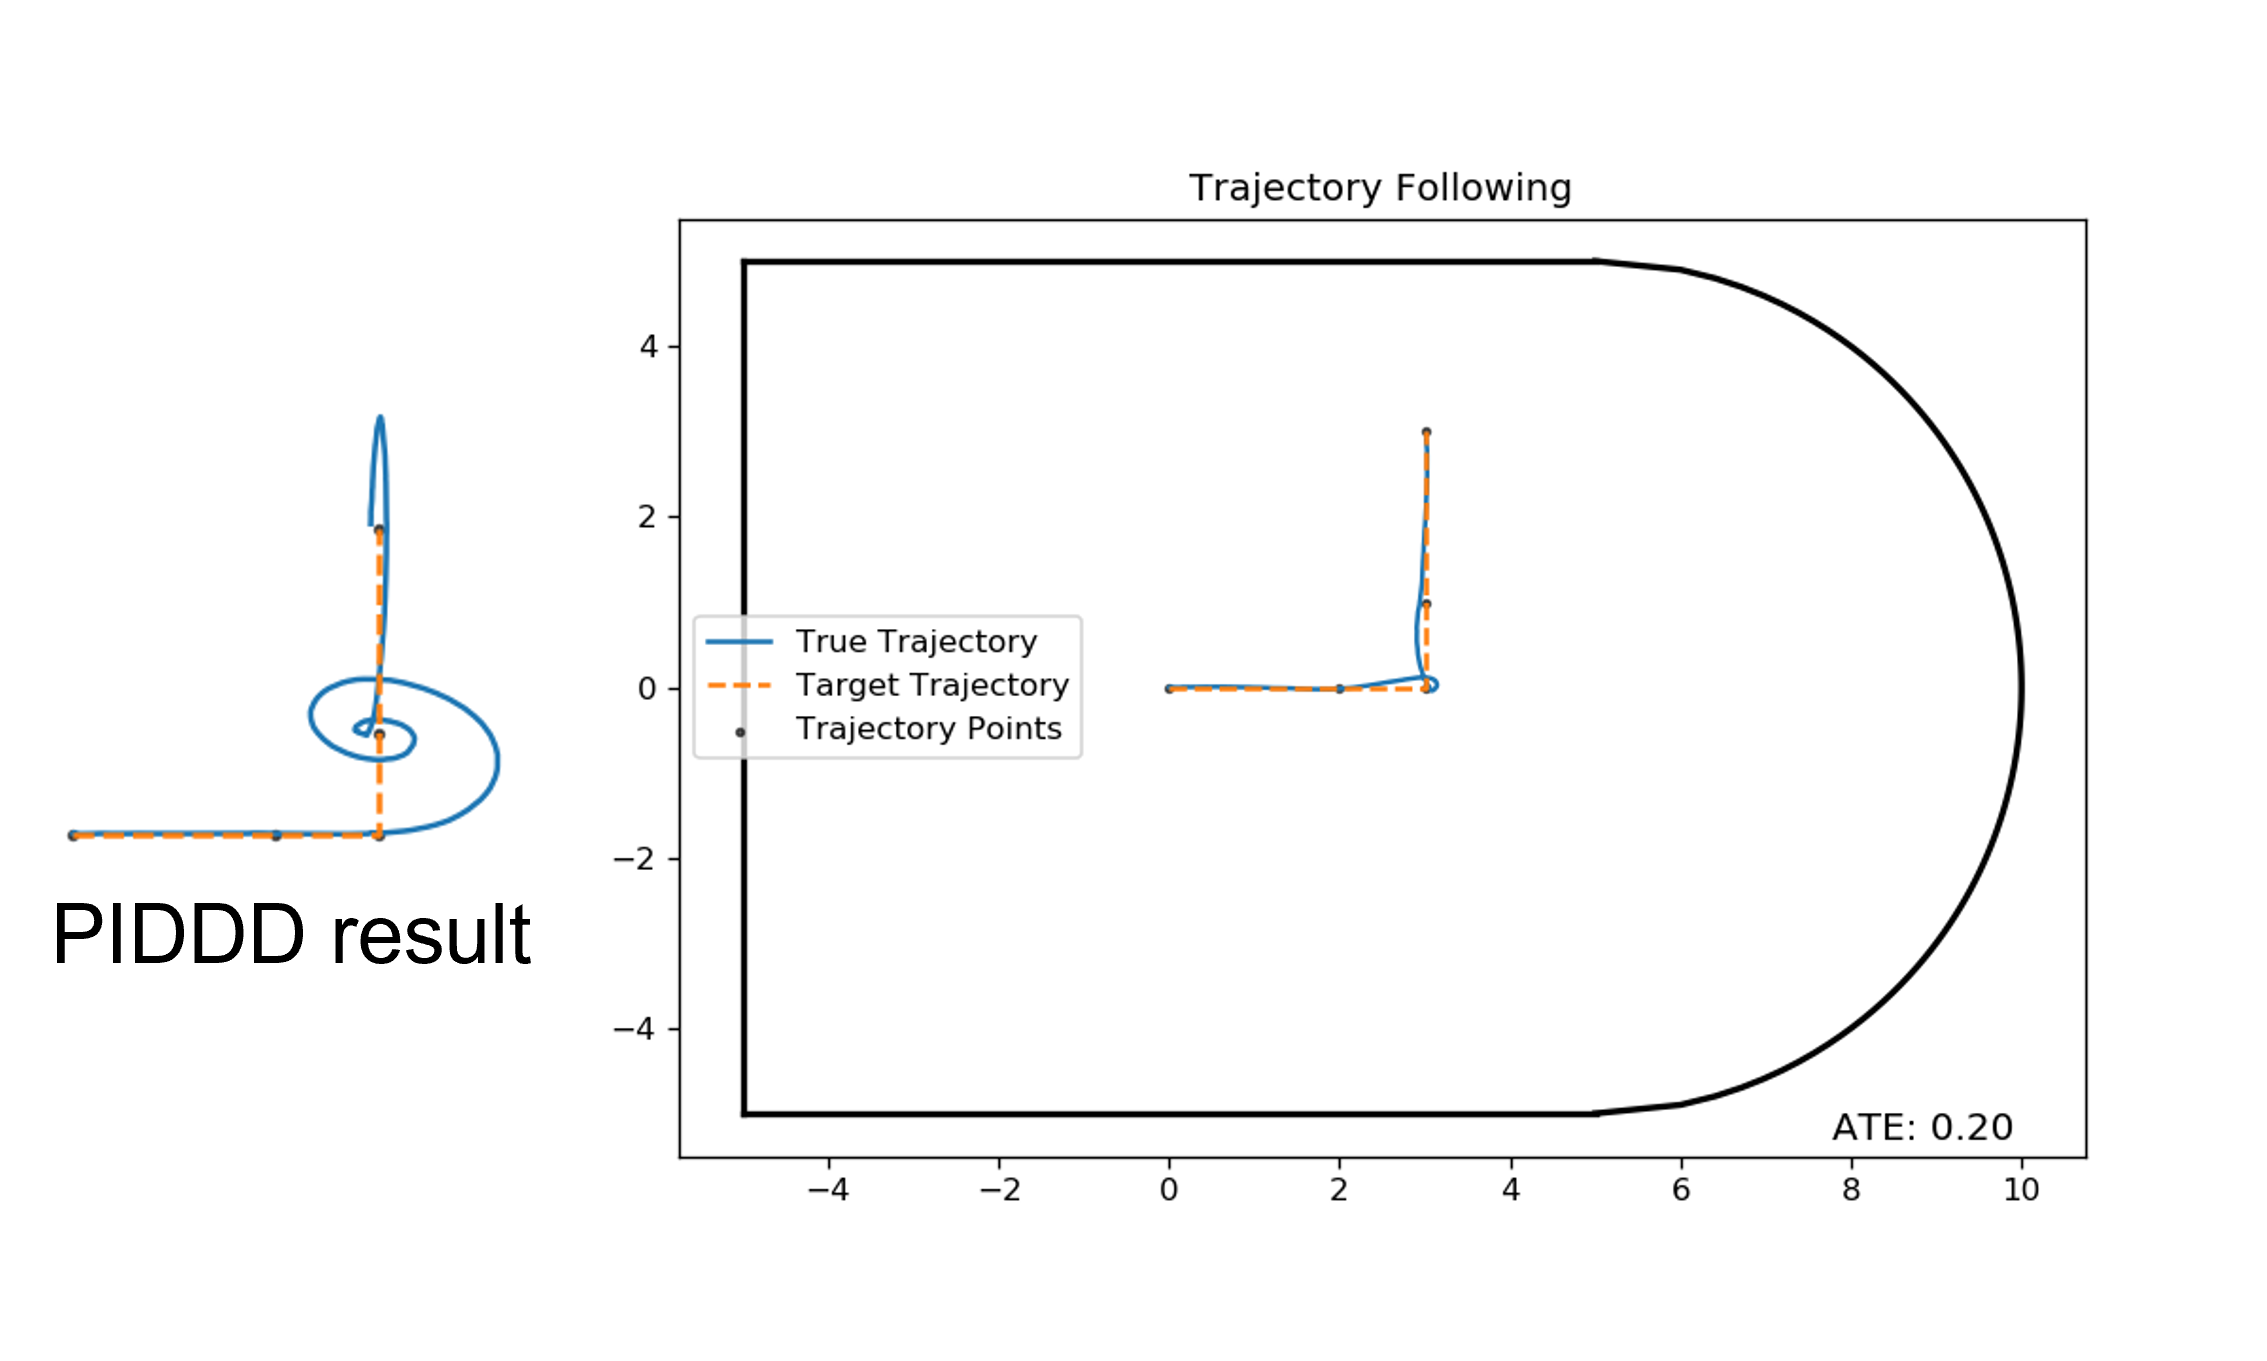
\includegraphics[width=0.6\linewidth]{assets/corner}
					\caption{快速过弯比较}
					\label{fig:corner}
				\end{figure}
			
			\subsubsection{其他轨迹结果}
				图\ref{fig:results}为三点匀速控制在其他轨迹上的结果。
			
				\begin{figure}[h!]
					\centering
					\begin{minipage}{0.5\textwidth}
						\adjustbox{valign=c}{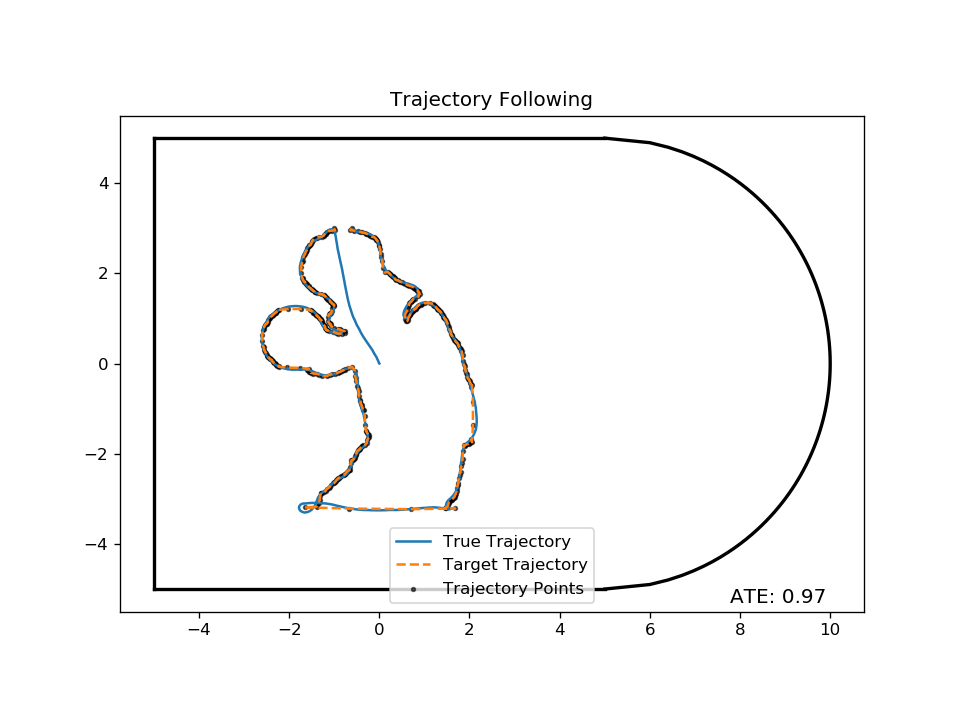
\includegraphics[width=\linewidth]{assets/fig_traj_kun1_adv.png}}
					\end{minipage}\hfill
					\begin{minipage}{0.5\textwidth}
						\adjustbox{valign=c}{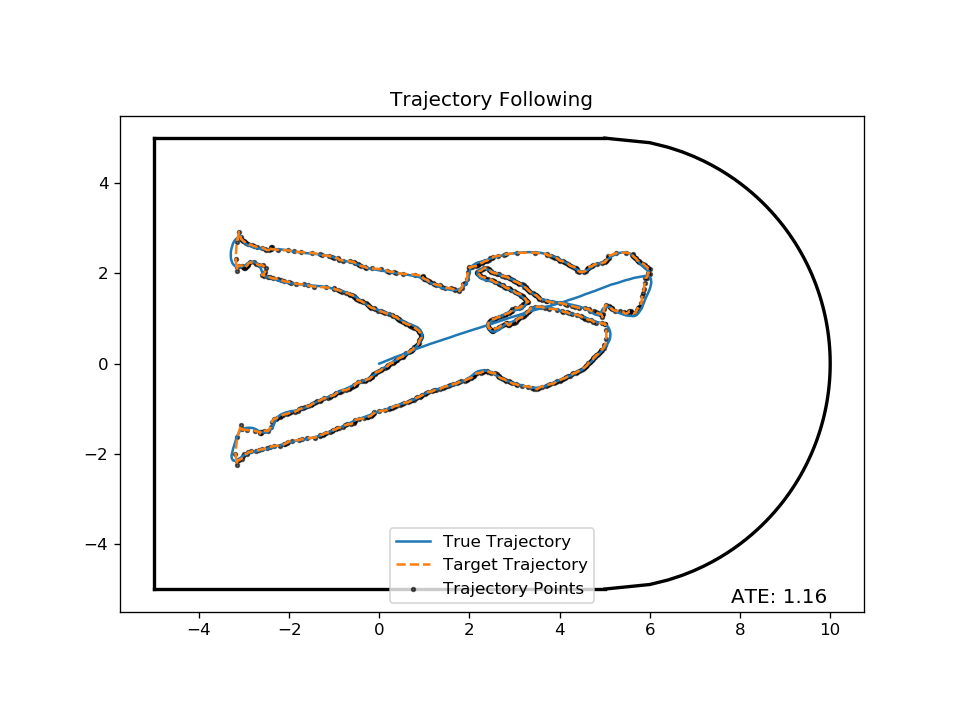
\includegraphics[width=\linewidth]{assets/fig_traj_kun2_adv.png}}
					\end{minipage}
					\caption{三点匀速控制 其他曲线}
					\label{fig:results}
				\end{figure}
		\subsection{速度控制比较}
			图\ref{fig:vt}展示了三点控制在不同速度的稳定性。速度提高时，稳定性趋于降低。我也尝试过提高机器人的质量，由于所有控制都是线性的，在\ref{ass}的假设下质量没有产生显著影响。
			
			\begin{figure}[h!]
				\centering
				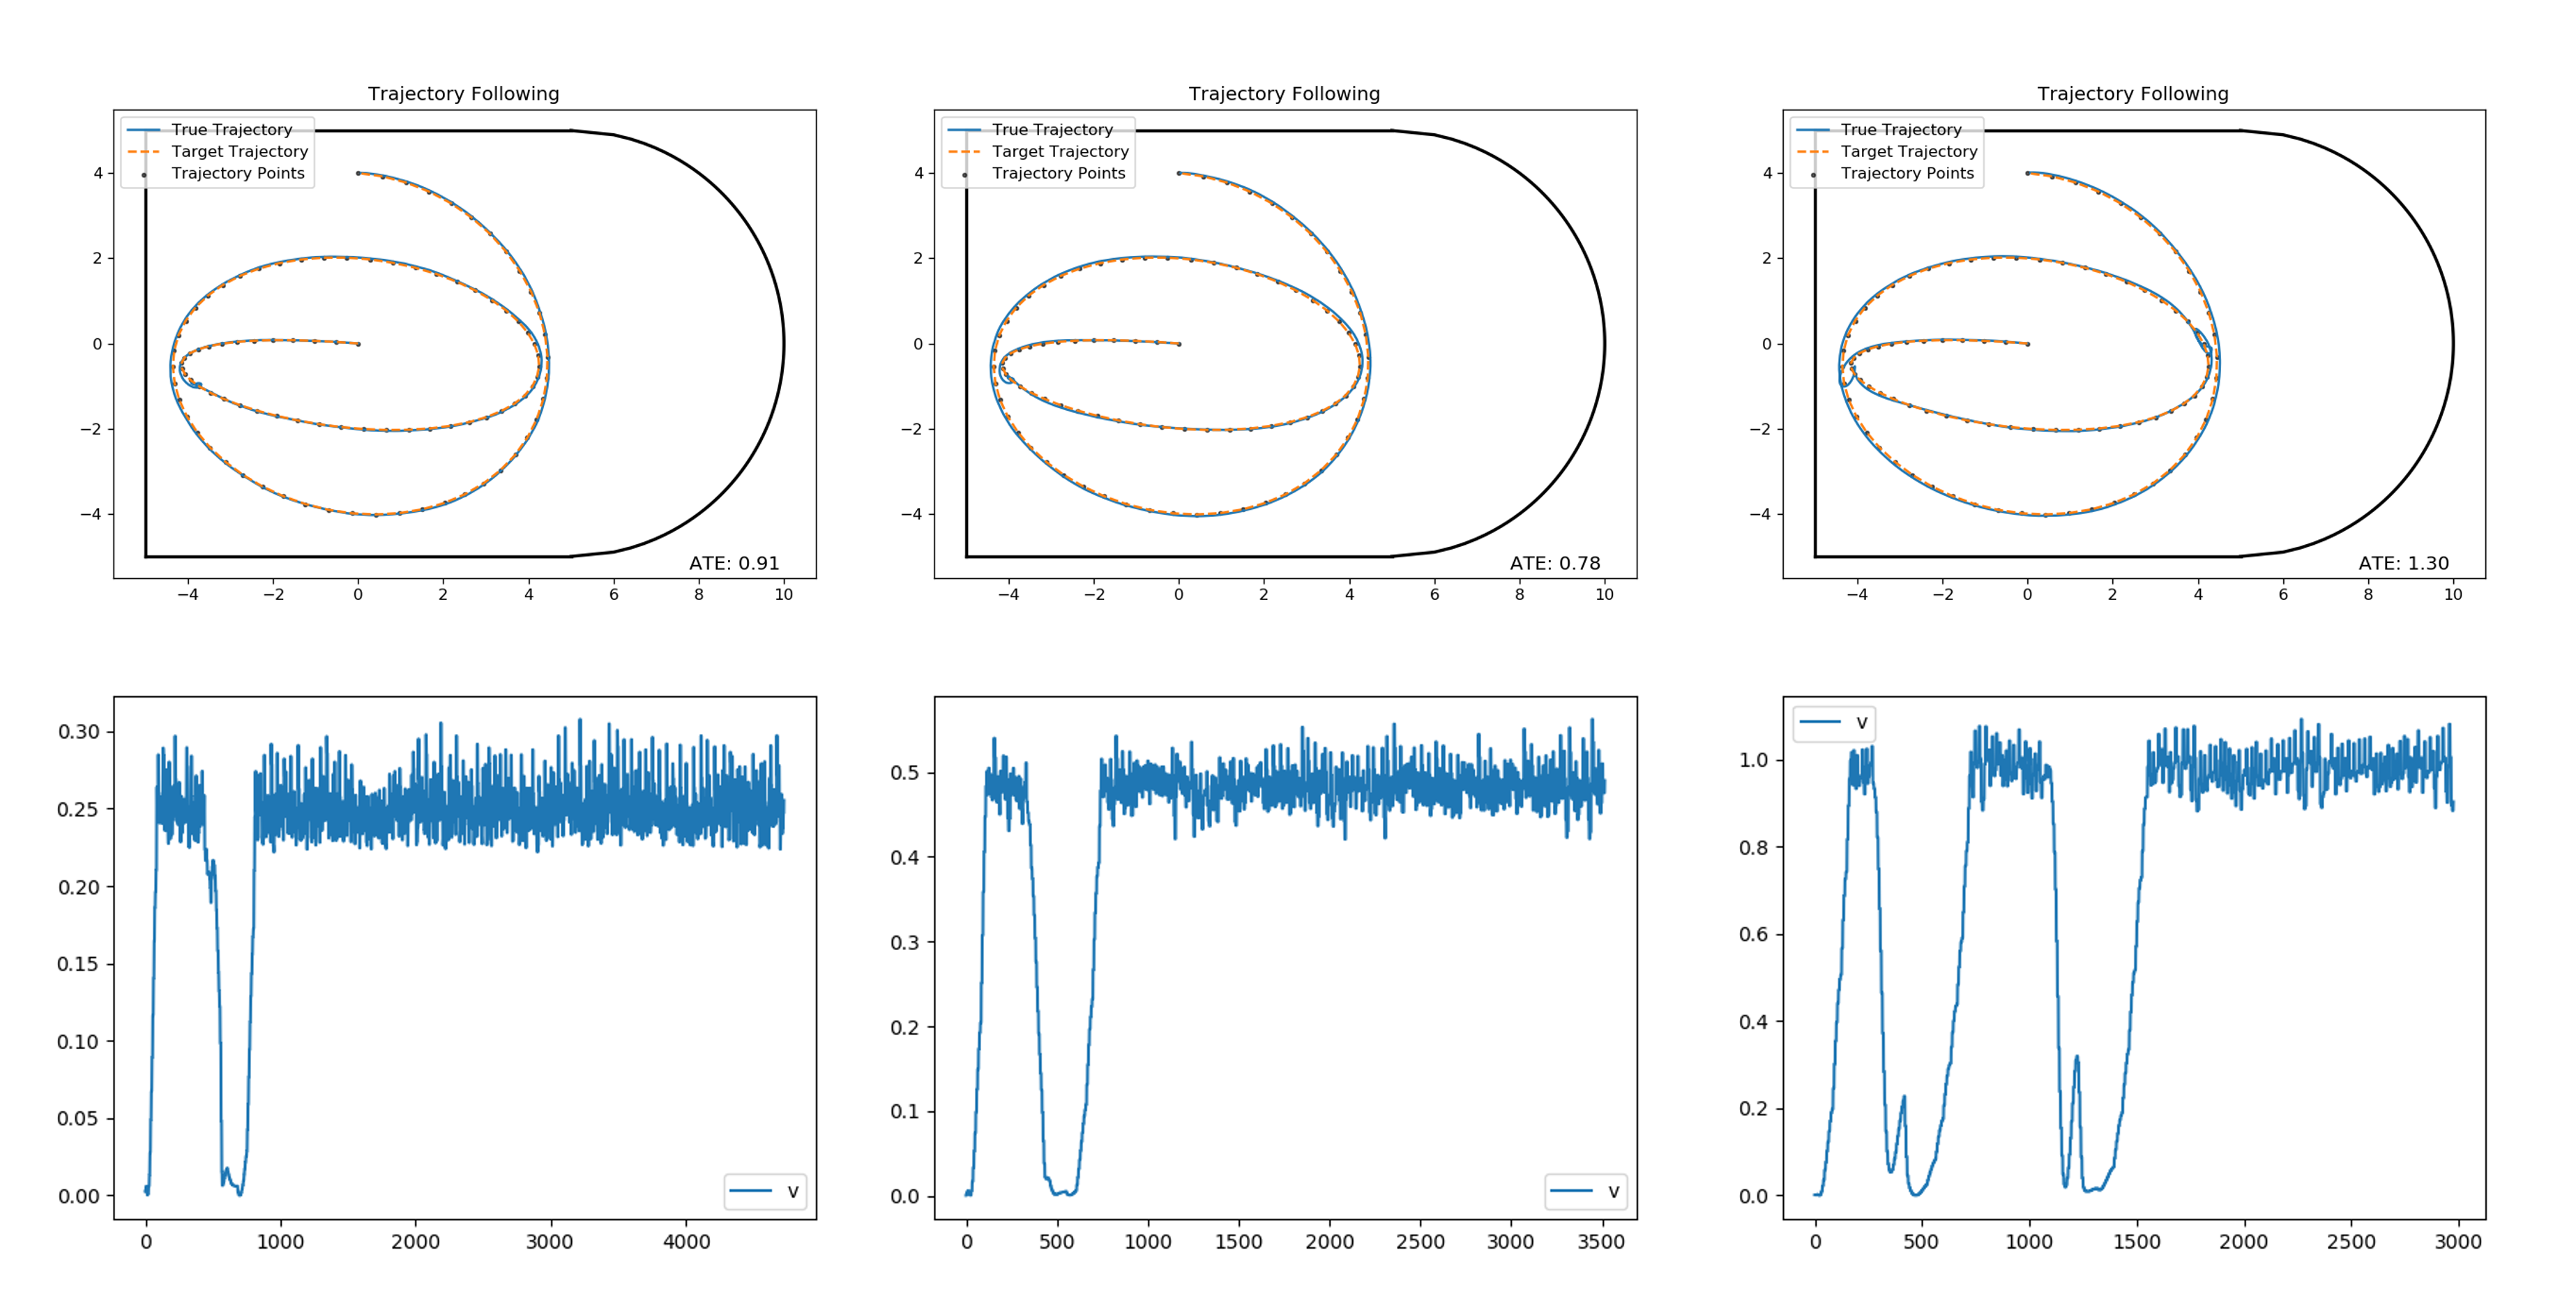
\includegraphics[width=0.7\linewidth]{assets/vt}
				\caption{速度控制比较}
				\label{fig:vt}
			\end{figure}
			
		\subsection{其他比较说明}
			由于PID类方法没有控制速度，且速度控制中稳定性和时间是trade off，难以公平的比较时间。且由于速度和轨迹都是不均匀的，定位点无法对齐，无法进行插值计算合理的ATE，故不进行量化比较。
		
	\section{对课程的意见与建议}
			希望可以提供设备。我了解到电院有空闲的机房教室，有可以流畅运行虚拟机的设备。考虑到我经历的恐怖的性能问题，建议考虑统一设备。

\end{document}


